\documentclass[11pt]{article}
\usepackage[margin=1in]{geometry}
\usepackage{amsmath,amssymb,amsthm,mathtools}
\usepackage{dsfont}
\usepackage{graphicx}
\usepackage{booktabs}
\usepackage{array}
\usepackage{placeins}
\usepackage[hyphens]{url}
\usepackage{microtype}
\usepackage{xcolor}
\usepackage{tikz}
\usetikzlibrary{arrows.meta,positioning,calc}
\usepackage{caption}
\captionsetup{font=small,labelfont=bf,margin=0.5em}
\usepackage[colorlinks=true,linkcolor=blue!55!black,citecolor=blue!55!black,urlcolor=blue!55!black]{hyperref}

\newcommand{\Tr}{\operatorname{Tr}}
\newcommand{\tr}{\operatorname{tr}}
\newcommand{\Np}{N'}
\newcommand{\one}{\mathds 1}
\newcommand{\ip}[2]{\langle #1,#2\rangle}
\newcommand{\eps}{\varepsilon}
\newcommand{\Dc}{\mathcal D}
\newcommand{\Dbar}{\bar{\mathcal D}}
\newcommand{\Vc}{\mathcal V}
\newcommand{\Wone}{W^{(1)}}
\newcommand{\dec}{\mathrm{dec}}
\newcommand{\sI}{s_{\rm in}}
\newcommand{\sout}{s_{\rm out}}
\newcommand{\qt}{\tilde q}
\newcommand{\Nh}{\hat N}
\newcommand{\poch}[2]{(#1;#2)_\infty}

% status tags (as in the previous reports)
\definecolor{cest}{RGB}{30,90,160}
\definecolor{cder}{RGB}{20,120,70}
\definecolor{cnum}{RGB}{150,90,10}
\definecolor{cconj}{RGB}{160,40,40}
\newcommand{\tagbox}[2]{\textsf{\small\color{#1}[#2]}}
\newcommand{\EST}{\tagbox{cest}{literature}}
\newcommand{\DER}{\tagbox{cder}{derived}}
\newcommand{\VER}{\tagbox{cder}{derived + verified}}
\newcommand{\NUM}{\tagbox{cnum}{numerical}}
\newcommand{\PRE}{\tagbox{cnum}{pre-registered}}
\newcommand{\INTERP}{\tagbox{cconj}{interpretation}}
\newcommand{\COND}{\tagbox{cconj}{derived under the chord rules}}

\theoremstyle{plain}
\newtheorem{theorem}{Theorem}
\newtheorem{proposition}{Proposition}
\newtheorem{lemma}{Lemma}
\newtheorem{corollary}{Corollary}
\theoremstyle{remark}
\newtheorem*{remark}{Remark}

\title{\bf The dressing spectrum from chords\\[6pt]\large Progress report, 14 October 2026}
\author{\texttt{syk\_gravity} project\\[2pt]\small Drafted by Claude for J.~Chryssanthacopoulos; results at commit
\texttt{097cd6e} (branch \texttt{t4-fourarc})}
\date{}

\emergencystretch=2em
\renewcommand{\topfraction}{0.9}
\renewcommand{\bottomfraction}{0.6}
\renewcommand{\textfraction}{0.08}
\renewcommand{\floatpagefraction}{0.8}
\numberwithin{equation}{section}

\begin{document}
\maketitle

\begin{abstract}
\noindent
The previous report reduced the decoder's localization to the distribution of \emph{dressing costs}: the eigenvalues
of the operator $\Dc=P\,E^\dagger H_0^{-1}E\,P$ on the BPS space of the smaller model, where $E$ is the pair-creation
operator of the added mode. $\Dc$ is a Euclidean-time-integrated, zero-temperature two-point function of a random
two-fermion matter operator. Here we compute it in the double-scaled chord theory of $\mathcal N=2$ SYK. Three results
are exact. (i) The BPS-to-continuum two-point function of a charged single-chord operator is the orthogonality measure
of the Al-Salam--Chihara polynomials, with parameters fixed by the two charges and the operator's dimension. Its
discrete part is the BPS-to-BPS result of Boruch, Lin and Yan; its Schwarzian limit is the $\mathcal N=2$ JT result of
Lin, Maldacena, Rozenberg and Shan. (ii) The time integral, i.e.\ the mean dressing cost, is a ${}_2\phi_1$. (iii) In
the chord theory, uncrossed matter-chord diagrams make the full dressing spectrum a free compound Poisson law. With no
fitted parameters, this gravitational answer reproduces the exact first-order heterogeneity $\Wone$ of the decoder to
$4$--$9\%$ for $\Np=10$--$16$, and the decoder's own $W$ to $-8\%$ to $+11\%$. We give a complete error budget.
Crossed diagrams contribute at most $0.5\%$ of the third moment. The free law is $3$--$5\%$ high because the exact
spectrum has a softer lower edge. The chord inputs add $1$--$3\%$. Predictions for the next size, $\Np=17$, are pre-registered.
Finally, the BPS states are \emph{not} equivalent at finite $N$, as the chord theory would have them. We show by an
exact sum rule that this heterogeneity is the microstate dependence of single-fermion BPS-to-BPS weights. It has an
incoherent part, which shrinks with $N$, and a coherent part, which does not.
\end{abstract}

\tableofcontents

%=====================================================================
\section{Introduction}\label{sec:intro}
%=====================================================================

\subsection{Where we stood}

The decoder of the uplift problem compares a BPS state of the $\Np$-mode model of one-flavor $\mathcal N=2$ SYK with the
BPS space of the $(\Np-1)$-mode model~\cite{CV,prog1013}. Its moments $T_{2m}=\langle y^m\rangle$, with $y=\cos^22\theta$
and $\theta$ the principal angle, obey the exact identity $T_4=T_2-W$, where $W=\langle y(1-y)\rangle$ is the weight at
intermediate angles~\cite[\S9]{prog1013}. Localization, the excess of the decoder's $T_4$ over an isotropic deformation
with the same $T_2$, is therefore a statement about $W$.

The previous report~\cite{prog1013} found an exact uplift map and, from it, the first-order decoder. To first order an
old BPS state $h$ is dressed by the cloud $-\eps Kh$, and its principal angle obeys $\tan^2\theta=\sigma^2$. Here
$\sigma^2$ is an eigenvalue of the \emph{dressing operator}
\begin{equation}\label{eq:D}
\Dc=P\,E^\dagger H_0^{-1}E\,P=\int_0^\infty d\tau\;P\,E^\dagger e^{-\tau H_0}E\,P ,
\end{equation}
acting on the old BPS space at charge $F$ (Prop.~5 of~\cite{prog1013}). $H_0$ is the old Hamiltonian, and
$E=\eta\wedge=\sum_I\eta_I\psi_I^\dagger$ creates a pair of fermions with the couplings $\eta$ of the added mode. The
first-order heterogeneity $\Wone$, computed from these dressing costs, reproduced the decoder's $W$ to $1$--$7\%$ for
$\Np=11$--$15$. It also passed a pre-registered test at $\Np=16$. The report closed by noting that $\Dc$ is a
time-integrated zero-temperature two-point function of a random two-fermion matter operator. Its spectrum is therefore
the kind of quantity the chord formalism of BLY~\cite{BLY} and BINT~\cite{BINT} computes.

\subsection{What this report does}

We carry out that computation and test it.
\begin{enumerate}\itemsep2pt
\item \textbf{The two-point function in closed form} (\S\ref{sec:asc}, \VER). Theorem~\ref{thm:asc}: the BPS-to-continuum
  spectral measure of a charged chiral single-chord operator is the Al-Salam--Chihara measure. It contains BLY's
  BPS-to-BPS formula as its point mass (Corollary~\ref{cor:bly}) and LMRS's super-Schwarzian formula as its
  triple-scaling limit (Corollary~\ref{cor:lmrs}).
\item \textbf{The time integral} (\S\ref{sec:time}, \VER). Proposition~\ref{prop:2phi1}: the mean dressing cost is a
  ${}_2\phi_1$, and it grows like $\lambda^{2\Delta-2}$ as $\lambda\to0$.
\item \textbf{The whole spectrum} (\S\ref{sec:diagrams}, \COND). Wick contractions of the couplings are matter-chord
  diagrams. Uncrossed diagrams sum to a free compound Poisson law (Proposition~\ref{prop:fcp}). Crossed diagrams are
  measured to be at most $0.5\%$ of the third moment \NUM.
\item \textbf{Gravity versus exact} (\S\ref{sec:tests}, \NUM). The chord prediction of $\Wone$ is $4$--$9\%$ high at
  $\Np=10$--$16$. We split the error into its sources and identify a soft lower edge of the exact spectrum.
\item \textbf{A pre-registered test at $\Np=17$} (\S\ref{sec:N17}, \PRE).
\item \textbf{BPS heterogeneity} (\S\ref{sec:hetero}). An exact sum rule (Proposition~\ref{prop:sumrule}) ties the
  part of the physics the chord theory misses to single-fermion BPS-to-BPS weights.
\end{enumerate}

%=====================================================================
\section{Setup}\label{sec:setup}
%=====================================================================

\subsection{The dressing problem}

The old model has $N=\Np-1$ complex fermions and supercharge $Q_0=\omega_0\wedge$ with a random $3$-form $\omega_0$
($p=3$, $E|C_{ijk}|^2=2$). Its BPS states at charge $F=\lfloor\Np/2\rfloor$ form the space $\mathcal B^F$ of dimension
$b_F$, with projector $P$. There are two dressing problems~\cite{prog1013}:
\begin{itemize}\itemsep1pt
\item the \textbf{$h$ family}: $\Dc=P\,E^\dagger G\,E\,P$ on $\mathcal B^F$, where $G=H_0^{-1}$ acts on the
  $e_{F+2}$ exact forms of degree $F+2$;
\item the \textbf{$g$ family}: $\Dc'=P'\,E\,G'E^\dagger P'$ on $\mathcal B^{F-1}$, where $G'=H_0^{-1}$ acts on the
  $e'_{F-3}$ coexact forms of degree $F-3$.
\end{itemize}
The pair operator $E=\sum_{i<j}\eta_{ij}c_i^\dagger c_j^\dagger$ has independent couplings with $E|\eta_{ij}|^2=2$. The
first-order decoder eigenvalues are $y=\big((1-s)/(1+s)\big)^2$ for $s\in\operatorname{spec}\Dc\cup\operatorname{spec}\Dc'$,
and $\Wone=\langle y(1-y)\rangle$ over all $b_F+b_{F-1}$ states. We call $s=\sigma^2$ the dressing cost. Two exact
facts fix the scale:
\begin{equation}\label{eq:c0}
\textstyle\sum_{i<j}\psi_{ij}\psi_{ij}^\dagger=\binom{N-F}{2}\ \text{on }\Lambda^F
\quad\Rightarrow\quad
E_\eta\langle h|E^\dagger E|h\rangle=c_0\equiv2\binom{N-F}{2},
\end{equation}
and likewise $c_0'=2\binom{F-1}{2}$ for the $g$ family. The normalized two-point function is
$G(\tau)=E_\eta\langle h|E^\dagger e^{-\tau H_0}E|h\rangle/c_0$, and the mean dressing cost is
$t_1=c_0\int_0^\infty G(\tau)\,d\tau$.

\subsection{Double-scaled chords at fixed charge}

We use the one-sided chord Hilbert space of BBNR~\cite[\S\S4.4--5.1]{BBNR}. A chord state is an alternating string of
chord ends, read from top to bottom:
\begin{gather*}
|\emptyset\rangle,\qquad |n,X\rangle=XOXO\cdots XO,\qquad |n,O\rangle=OXOX\cdots OX\qquad(\text{length }2n),\\
|n{+}\tfrac12,X\rangle=XOX\cdots X,\qquad |n{+}\tfrac12,O\rangle=OXO\cdots O\qquad(\text{length }2n+1).
\end{gather*}
At fixed charge $s$, $Q$ opens an $O$ chord at the bottom with weight $q^{s}$ and closes $X$ chords. $Q^\dagger$ opens
$X$ with $q^{-s}$ and closes $O$. Non-alternating strings are null. The inner product is BBNR (4.37), and $T=QQ^\dagger+Q^\dagger Q$.
Here $q=e^{-\lambda}$ and $\lambda=2p^2/N$. The chord charge of a fermion-number sector of degree $d$ is $s=(d-N/2)/p$.
Applied to the states we need, these rules give
\begin{align}
Q|n,X\rangle&=-q^{n-1}|n{-}\tfrac12,O\rangle, & Q|n,O\rangle&=q^{s}|n{+}\tfrac12,O\rangle+q^{-1}|n{-}\tfrac12,O\rangle,\label{eq:Qrules}\\
Q|\emptyset\rangle&=q^{s}|\tfrac12,O\rangle, & Q|n{+}\tfrac12,O\rangle&=0,\nonumber\\
Q|\tfrac12,X\rangle&=q^s|1,X\rangle+|\emptyset\rangle, & Q|n{+}\tfrac12,X\rangle&=q^{s}|n{+}1,X\rangle+|n,X\rangle+q^{n}|n,O\rangle\quad(n\ge1),\nonumber
\end{align}
with $Q^\dagger$ obtained by exchanging $O\leftrightarrow X$ and $s\to-s$. The norms are
\begin{gather}
\langle n,O|n,O\rangle=\langle n,X|n,X\rangle=q^{-n}(q^2;q^2)_{n-1},\qquad \langle n,O|n,X\rangle=-(q^2;q^2)_{n-1},\label{eq:gram}\\
\langle n{+}\tfrac12,X|n{+}\tfrac12,X\rangle=q^{s-n}(q^2;q^2)_n,\qquad \langle n{+}\tfrac12,O|n{+}\tfrac12,O\rangle=q^{-s-n}(q^2;q^2)_n .\nonumber
\end{gather}
\EST\ These follow from BBNR (4.16)--(4.17) and (4.37). We checked them in a transfer-matrix implementation
(\path{src/chord_transfer.py}), which reproduces BBNR (4.40)--(4.42) and (5.5), BLY (3.17) and BLY (4.7).

The bosonic sector splits into the $T$-invariant families $\mathcal B=Q\,\mathcal F$ (exact) and
$\bar{\mathcal B}=Q^\dagger\mathcal F$ (coexact). For $|s|<\tfrac12$ there is in addition a unique zero mode $\Psi_s$, the
supersymmetric Hartle--Hawking state of BLY. On $\mathcal B$, with $b_n=Q|n{+}\tfrac12,X\rangle$, BBNR (5.5) reads
$Tb_n=q^{-1}(1-q^{2n})b_{n-1}+(q^{-s}+q^{s-1})b_n+b_{n+1}$. Its spectrum is
\begin{equation}\label{eq:Lambda}
\Lambda_s(\phi)=2q^{-1/2}\big[\cosh\lambda(s-\tfrac12)-\cos\phi\big],\qquad \phi\in(0,\pi),
\end{equation}
gapped unless $s=\tfrac12$.

\begin{remark}[A sign in BBNR]
The eigenvector of~\eqref{eq:Lambda} is $v(\phi)=\sum_n\alpha_n(\phi)b_n$ with
$\alpha_n=q^{n/2}H_n(-\cos\phi\,|\,q^2)/(q^2;q^2)_n$, where $H_n$ are the continuous $q$-Hermite polynomials. BBNR
(5.10) writes $H_n(+\cos\phi|q^2)$. That is the eigenvector for $+\cos\phi$ in~\eqref{eq:Lambda}, which can be checked
directly from (5.5). The slip is harmless for everything in BBNR, because their measure is symmetric under
$\phi\to\pi-\phi$. It matters for kernels with one BPS end, which are not symmetric. Combining (5.10) with (5.3)
naively reflects the BPS-to-continuum weight from the bottom to the top of the band.
\end{remark}

The normalization is $\langle\emptyset|v(\phi)\rangle=1$ and
$\langle v(\phi)|v(\phi')\rangle=q^s\Lambda_s(\phi)\,2\pi\delta(\phi-\phi')/\poch{q^2,e^{\pm2i\phi}}{q^2}$
(BBNR 5.11). The $\mathcal B$-family density at charge $s$ is therefore
\begin{equation}\label{eq:rhoB}
\rho_B(\phi)=\frac{\poch{q^2,e^{\pm2i\phi}}{q^2}\,q^{-s}}{2\pi\,\Lambda_s(\phi)} .
\end{equation}

\subsection{Charged matter}

A chiral single-chord operator built from $p'$ fermions (BBNR \S7.1) changes the charge of the region it encloses by
$\delta=p'/p$. It also inserts $\qt^{\Nh}$ at the junction, where $\qt=q^{\delta}$ and $\Nh|n,\cdot\rangle=n|n,\cdot\rangle$.
In BLY's language the operator has dimension $\Delta=\delta/2$. For the pair operator, $p'=2$, so $\delta=\tfrac23$ and
$\Delta=\tfrac13$. The $h$ family starts at $\sout=(F-N/2)/p$ and ends at $\sI=\sout+\delta$. The $g$ family is its mirror
image under $s\to-s$. For even $\Np$ both families have $(\sout,\sI)=(\tfrac16,\tfrac56)$. For odd $\Np$, $h$ has
$(0,\tfrac23)$ and $g$ has $(\tfrac13,1)$. In every case $\sI>\tfrac12$: the target sector has no BPS states.

We compare with finite $N$ at $\lambda=2p^2/N$, where $N=\Np-1$ is the size of the old model. The energy scale $\kappa$
($H_0\leftrightarrow\kappa T$) is fixed by the exact first moment of $H_0$ in the target sector,
$\kappa=2[\binom{d}{3}+\binom{N-d}{3}]/(q^{\sI}+q^{-\sI})$, with $d=F+2$ for $h$ and $d=F-3$ for $g$. The overall
normalization is the exact $c_0$ of~\eqref{eq:c0}. Nothing is fitted.

%=====================================================================
\section{The BPS-to-continuum two-point function}\label{sec:asc}
%=====================================================================

\begin{theorem}[Closed form]\label{thm:asc}\VER\
Let $|\sout|<\tfrac12$ and $\sI=\sout+\delta>\tfrac12$, and let $\Psi$ be the zero mode at charge $\sout$. The normalized
two-point function $G(\tau)=\langle\emptyset|e^{-\tau\kappa T_{\rm in}}\qt^{\Nh}|\Psi\rangle/\langle\emptyset|\Psi\rangle$
is
\begin{equation}\label{eq:asc}
\begin{gathered}
G(\tau)=\int_0^\pi d\phi\,f(\phi)\,e^{-\tau\kappa\Lambda_{\sI}(\phi)},\qquad
f(\phi)=\frac{\poch{ab}{q^2}\,\poch{q^2,e^{\pm2i\phi}}{q^2}}{2\pi\,\poch{ae^{\pm i\phi},\,be^{\pm i\phi}}{q^2}},\\
a=q^{\sI-\frac12},\qquad b=q^{\frac12+\delta-\sout}.
\end{gathered}
\end{equation}
This is the normalized orthogonality measure of the Al-Salam--Chihara polynomials in $x=\cos\phi$, with base $q^2$ and
parameters $(a,b)$~\cite{KLS}. Equivalently $f=\rho_B\,A$, with the squared matrix element
\begin{equation}\label{eq:A}
A(\phi)=\frac{\langle v(\phi)|\qt^{\Nh}|\Psi\rangle}{\langle\emptyset|\Psi\rangle}
=\frac{\poch{q^{2\delta}}{q^2}}{\poch{q^{\sI+\frac32}e^{\pm i\phi},\ q^{\frac12+\delta-\sout}e^{\pm i\phi}}{q^2}} .
\end{equation}
\end{theorem}

The proof has four steps.

\paragraph{Step 1: the BPS state.} Write
$\Psi=|\emptyset\rangle+\sum_{m\ge1}\big(x_m|m,X\rangle+o_m|m,O\rangle\big)$ and set $x_0=o_0=1$. By~\eqref{eq:Qrules},
$Q\Psi=0$ and $Q^\dagger\Psi=0$ read, coefficient by coefficient,
\begin{equation}\label{eq:gsrec}
q^{s}o_m+q^{-1}o_{m+1}-q^mx_{m+1}=0,\qquad q^{-s}x_m+q^{-1}x_{m+1}-q^mo_{m+1}=0\qquad(m\ge0).
\end{equation}
The solution is $x_m=q^{3m/2}H_m(-\cosh\lambda(s+\tfrac12)\,|\,q^2)/(q^2;q^2)_m$ (and $o_m$ is the same with $s\to-s$).
These are BLY's amplitudes (3.6)--(3.7) in BBNR's normalization. We checked them against the zero mode of the transfer
matrix to $10^{-14}$.

\paragraph{Step 2: the matter overlap.} Opening an $X$ chord carries $q^{-s}$, so
$Q^\dagger_{\rm in}=q^{-\delta}\,Q^\dagger_{\rm out,open}+Q^\dagger_{\rm close}$. The closing part does not depend on the
charge. Let $Q^\dagger_{\rm in}$ act on $\qt^{\Nh}\Psi$. The coefficient of $|m{+}\frac12,X\rangle$ receives three
contributions: the opening term from $|m,X\rangle$, and the closing terms from $|m{+}1,X\rangle$ and $|m{+}1,O\rangle$.
Using the second relation in~\eqref{eq:gsrec}, which is $Q^\dagger_{\rm out}\Psi=0$, it equals
$\qt^m x_m\,(q^{-\sI}-\qt\,q^{-\sout})$. Multiplying by the norm~\eqref{eq:gram} gives
\begin{equation}\label{eq:overlap}
\langle b_m|\qt^{\Nh}|\Psi\rangle=\langle m{+}\tfrac12,X|Q^\dagger_{\rm in}\qt^{\Nh}\Psi\rangle
=(1-\qt\,q^{\delta})\,(\qt/q)^m\,(q^2;q^2)_m\,x_m .
\end{equation}
A BPS state is annihilated by $Q^\dagger$. That is what turns a two-dimensional sum over chord states into this single
sequence.

\paragraph{Step 3: $q$-Mehler.} Combine~\eqref{eq:overlap} with $\alpha_m(\phi)$ and set $\qt=q^\delta$:
\[
A(\phi)=(1-q^{2\delta})\sum_{m\ge0}\frac{H_m(-\cos\phi|q^2)\,H_m(-\cosh\lambda(\sout+\tfrac12)|q^2)}{(q^2;q^2)_m}\,(q^{1+\delta})^m .
\]
The $q$-Mehler (Rogers) formula~\cite{GR,KLS},
\[
\sum_{m\ge0}\frac{H_m(\cos\theta|Q)\,H_m(\cos\psi|Q)}{(Q;Q)_m}\,t^m=\frac{\poch{t^2}{Q}}{\poch{te^{i(\pm\theta\pm\psi)}}{Q}},
\]
applies with $Q=q^2$, $t=q^{1+\delta}$, $e^{i\theta}=-e^{-i\phi}$ and $e^{i\psi}=-q^{\sout+\frac12}$. The series converges
because $tq^{-\sout-\frac12}=b<1$. The result is~\eqref{eq:A}.

\paragraph{Step 4: a cancellation.} Note that $q^{-\sI}/\Lambda_{\sI}(\phi)=1/|1-ae^{i\phi}|^2$, and that the first
denominator parameter of~\eqref{eq:A} is $q^{\sI+3/2}=aq^2$. Hence
$(1-ae^{\pm i\phi})\poch{aq^2e^{\pm i\phi}}{q^2}=\poch{ae^{\pm i\phi}}{q^2}$, and $f=\rho_BA$ collapses
to~\eqref{eq:asc}. Since $ab=q^{2\delta}$ and $\poch{q^{2\delta}}{q^2}=(1-q^{2\delta})\poch{q^{2+2\delta}}{q^2}$, the
prefactor is exactly the normalization of the Al-Salam--Chihara measure, $\int f\,d\phi=1$~\cite{KLS}. \qed

\paragraph{Checks.} The closed form was compared with the transfer-matrix engine (exact chord rules, $\ell_{\max}=200$--$400$).
The moments $\int f\Lambda^k$ for $k=-2,\dots,3$ agree to $10^{-15}$ at several values of $(\lambda,\sout,\delta)$
(\path{tests/test_chord_dressing.py}). The negative moments include the time integral of the next section.

\begin{corollary}[BPS-to-BPS weight = BLY]\label{cor:bly}\VER\
Continue~\eqref{eq:asc} to $\sI<\tfrac12$, where the target sector has BPS states. Then $a>1$, and the
Al-Salam--Chihara measure acquires a point mass at $x=(a+a^{-1})/2$, i.e.\ at zero energy. Its weight is
\[
\frac{\poch{a^{-2}}{q^2}}{\poch{b/a}{q^2}}=\frac{\poch{q^{1-2\sI}}{q^2}}{\poch{q^{1-2\sout}}{q^2}} .
\]
This equals the normalized BPS-to-BPS weight of BLY (4.14), multiplied by $\sqrt{D(\sI)/D(\sout)}$ to convert between
normalizations.
\end{corollary}
We checked the point mass three ways, at four parameter points, to $10^{-12}$: as one minus the continuous part, as the
engine's zero-mode weight, and against BLY (4.14). The discrete and continuous parts of the zero-temperature two-point
function of a charged chiral operator are thus one object. BLY computed the first; Theorem~\ref{thm:asc} supplies the
second.

\begin{corollary}[Schwarzian limit = LMRS]\label{cor:lmrs}\DER\
Set $\phi=\lambda k$ and let $\lambda\to0$, using $\poch{Q^{x}}{Q}\to\poch{Q}{Q}(1-Q)^{1-x}/\Gamma(x)$. Then
\begin{equation}\label{eq:schw}
f\,d\phi\ \propto\ k\sinh(\pi k)\,\Big|\Gamma\big(\Delta-\tfrac14+\tfrac{\sout}{2}+\tfrac{ik}{2}\big)\,
\Gamma\big(\Delta+\tfrac14-\tfrac{\sout}{2}+\tfrac{ik}{2}\big)\Big|^2dk .
\end{equation}
This is the zero-energy-to-continuum term (43) of LMRS~\cite{LMRS}, with $j'=\sout$, $j=\sI$ and $s=k/2$.
\end{corollary}
To see the match, use $|\Gamma(z+1)|^2=|z|^2|\Gamma(z)|^2$ with $z=\Delta-\frac14+\frac{\sout}2+\frac{ik}2$, and note
that $|z|^2\propto\Lambda$ in this limit. LMRS's measure $s\sinh 2\pi s/E_{s,j}$ times their
$\Gamma(\Delta+\frac12\pm\frac{2j'+1}4\pm is)$ is then~\eqref{eq:schw}. Theorem~\ref{thm:asc} is thus the
$q$-deformation of the $\mathcal N=2$ JT gravity answer, just as BLY found for the BPS-to-BPS piece.

\paragraph{Literature.} BLY~\cite{BLY} computed the BPS-to-BPS weights (their \S4). BBNR (7.17)~\cite{BBNR} give the
moments between ground states and the continuum, integrated over the charge. We have not found in BBNR, BLY or
LMRS the fixed-charge measure~\eqref{eq:asc}, its Al-Salam--Chihara form, or the time integral of the next section.

\begin{figure}[t]
\centering
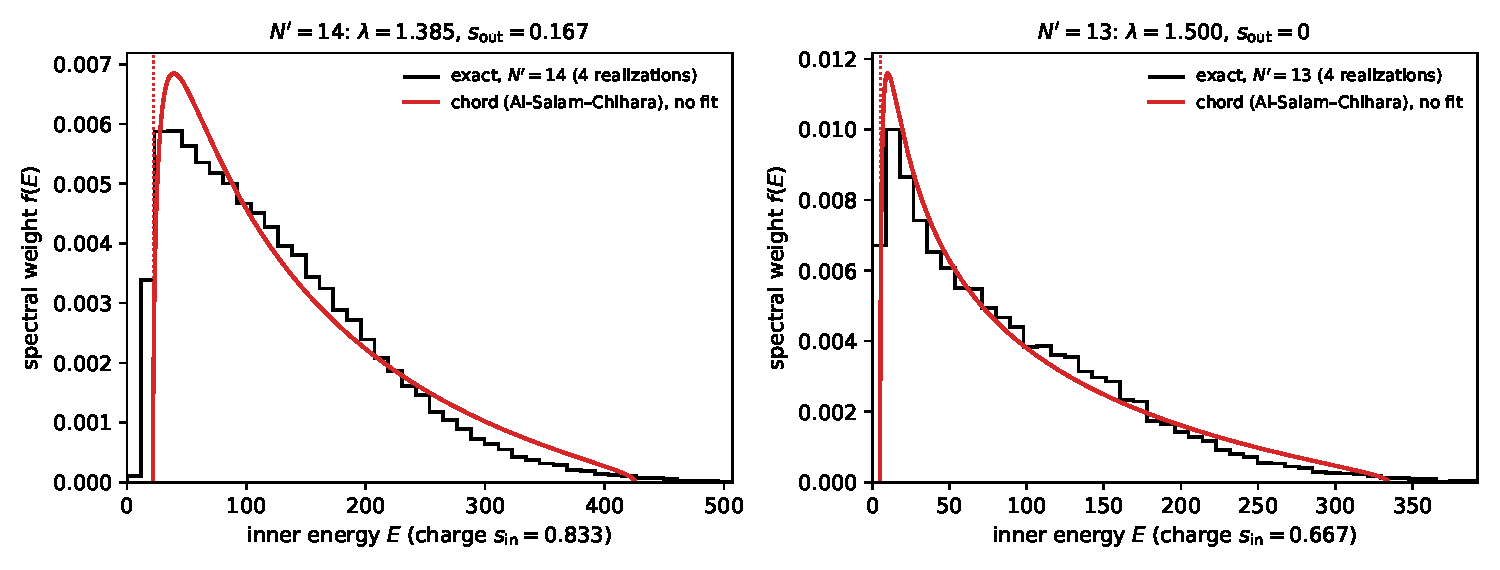
\includegraphics[width=\textwidth]{progress_2026-10-14_figs/fig_weight.pdf}
\caption{BPS-to-continuum spectral weight of the pair operator, $f(E)$ with $E=\kappa\Lambda_{\sI}$, for the $h$
family. Black: exact old models at $\Np=14$ and $13$ (four realizations; weight $\Vc_{nn}/(b\,c_0)$ of each inner
level, binned). Red: Theorem~\ref{thm:asc} at $\lambda=2p^2/N$, $\kappa$ from the first moment, no fit. The dotted line
is the double-scaled gap. The bulk agrees. The finite-$p$ spectrum is broader and leaks below the gap, which matters for
the $1/E$-weighted dressing cost.}
\label{fig:weight}
\end{figure}

%=====================================================================
\section{The time-integrated two-point function}\label{sec:time}
%=====================================================================

\begin{proposition}[Mean dressing cost]\label{prop:2phi1}\VER\
Under the hypotheses of Theorem~\ref{thm:asc},
\begin{equation}\label{eq:2phi1}
\int_0^\infty G(\tau)\,d\tau=\frac1\kappa\int_0^\pi\frac{f(\phi)}{\Lambda_{\sI}(\phi)}d\phi
=\frac1\kappa\,\frac{q^{\sI}}{1-q^{2\delta}}\;{}_2\phi_1\!\left(q^2,q^2;\,q^{2+2\delta};\,q^2,\,q^{2\sI-1}\right),
\end{equation}
and the mean first-order dressing cost is $t_1=c_0\int_0^\infty G\,d\tau$.
\end{proposition}

\begin{proof}
We have $\Lambda_{\sI}=q^{-1/2}(a+a^{-1}-2x)$, so the integral is $\frac{q^{1/2}}2F(x_a)$, where
$F(z)=\int d\mu(x)/(z-x)$ is the Stieltjes transform of the Al-Salam--Chihara measure $\mu$ and $x_a=(a+a^{-1})/2>1$.
Let $p_n$ be the monic orthogonal polynomials. They satisfy
$xp_n=p_{n+1}+\frac{a+b}2Q^np_n+\gamma_np_{n-1}$ with $Q=q^2$ and $\gamma_n=\frac14(1-Q^n)(1-abQ^{n-1})$~\cite{KLS}.
Let $q_n$ be the second-kind functions, which form the minimal solution of the same recursion. The Casoratian
$W_n=p_nq_{n-1}-p_{n-1}q_n$ obeys $W_{n+1}=\gamma_nW_n$ with $W_1=1$. Telescoping $q_n/p_n-q_{n+1}/p_{n+1}=W_{n+1}/(p_np_{n+1})$
and using $q_n/p_n\to0$ gives
\[
F(z)=\sum_{n\ge0}\frac{\gamma_1\cdots\gamma_n}{p_n(z)\,p_{n+1}(z)} .
\]
At $z=x_a$ the ${}_3\phi_2$ representation of the polynomials has the parameter $ae^{-i\theta}=1$, so it truncates to
its first term: $p_n(x_a)=(ab;Q)_n/(2a)^n$. These grow like $a^{-n}$, so they are dominant, as required. Substituting,
the $n$-th term is $2a\,a^{2n}(Q;Q)_n/(ab;Q)_{n+1}$. Summing gives
$F(x_a)=\frac{2a}{1-ab}\,{}_2\phi_1(Q,Q;abQ;Q,a^2)$, and $q^{1/2}a=q^{\sI}$.
\end{proof}

The ${}_2\phi_1$ agrees with direct quadrature to $10^{-15}$. As $\lambda\to0$, $(Q;Q)_n/(Q^{1+\delta};Q)_n\to\Gamma(1+\delta)n^{-\delta}$
and $1-a^2\simeq\lambda(2\sI-1)$, so
\begin{equation}\label{eq:smalllam}
\int_0^\pi\frac{f}{\Lambda_{\sI}}\,d\phi\simeq\frac{\pi}{2\sin\pi\delta}\,\lambda^{\delta-2}\,(2\sI-1)^{\delta-1}.
\end{equation}
The integral is dominated by the near-gap (Schwarzian) region. With $c_0/\kappa\simeq\lambda/p$ at large $N$, the
double-scaled mean dressing cost grows like $t_1\propto\lambda^{\delta-1}\propto N^{1/3}$ for the pair operator.

\begin{figure}[t]
\centering
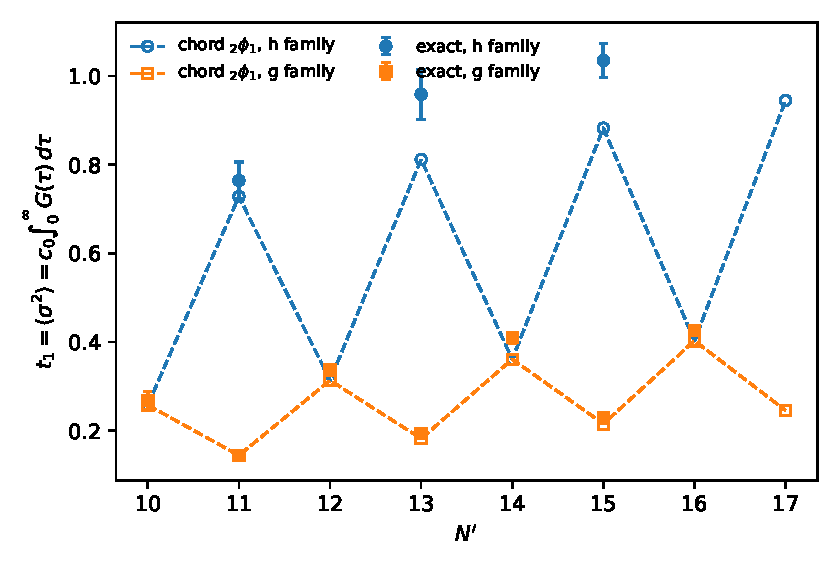
\includegraphics[width=0.62\textwidth]{progress_2026-10-14_figs/fig_t1.pdf}
\caption{Mean first-order dressing cost. Filled symbols: exact (mean $\pm$ SE over 2--4 realizations). Open symbols:
Proposition~\ref{prop:2phi1}, no fit. The alternation with parity comes from the target charge: at odd $\Np$ the $h$
family lands at $\sI=\frac23$, close to the gapless sector $\sI=\frac12$, and the $g$ family at $\sI=1$.}
\label{fig:t1}
\end{figure}

\paragraph{Comparison with finite $N$} \NUM. Table~\ref{tab:t1} and Figure~\ref{fig:t1} compare $t_1$ with the exact
old models. The chord theory reproduces the parity alternation and the size of $t_1$. It is low by $4$--$15\%$ in the
$h$ family and by $0$--$6\%$ in the $g$ family. The deficit is largest at odd $\Np$, where the gap is small.
Figure~\ref{fig:weight} shows the reason. The exact spectrum of the charged sector is broader than the double-scaled one
(squared coefficient of variation $0.36$--$0.41$ against $0.32$--$0.36$), and it extends below the double-scaled gap
(lowest level $13.4$ against $21.9$ at $\Np=14$). The time integral weights this tail by $1/E$. Recalibrating $\lambda$
does not help: at $\Np=14$ the exact spectrum is as broad as the broadest chord spectrum at this charge. This is a
finite-$p$ effect ($p=3$).

\begin{table}[ht]
\centering\small
\caption{Mean dressing cost $t_1$: exact (mean $\pm$ SE over realizations) and Proposition~\ref{prop:2phi1}. Also
listed: the fraction of $\|S\|_F^2$ on the diagonal of $S=G^{1/2}\Vc G^{1/2}$ in the inner energy basis
(\S\ref{sec:diagrams}), and the lowest inner energy.}
\label{tab:t1}
\setlength{\tabcolsep}{5pt}
\begin{tabular}{lcccccc}\toprule
$\Np$, fam. & real. & $t_1$ exact & $t_1$ chord & chord/exact & diag.\ frac.\ of $S$ & $E_{\min}$ exact / chord gap\\\midrule
10, $h$ (= $g$) & 4 & $0.268\pm0.020$ & 0.258 & 0.96 & 0.9980 & 15.3 / 16.0\\
11, $h$ & 4 & $0.764\pm0.042$ & 0.728 & 0.95 & 0.9969 & 3.4 / 4.4\\
11, $g$ & 4 & $0.144\pm0.010$ & 0.144 & 1.00 & 0.9885 & 40.6 / 38.4\\
12, $h$ (= $g$) & 4 & $0.337\pm0.007$ & 0.314 & 0.93 & 0.9967 & 14.1 / 18.9\\
13, $h$ & 4 & $0.959\pm0.057$ & 0.812 & 0.85 & 0.9948 & 2.8 / 5.2\\
13, $g$ & 4 & $0.194\pm0.008$ & 0.182 & 0.94 & 0.9862 & 35.4 / 45.1\\
14, $h$ (= $g$) & 4 & $0.410\pm0.012$ & 0.361 & 0.88 & 0.9952 & 13.4 / 21.9\\
15, $h$ & 3 & $1.035\pm0.039$ & 0.882 & 0.85 & 0.9936 & 3.1 / 5.9\\
15, $g$ & 3 & $0.228\pm0.005$ & 0.216 & 0.94 & 0.9853 & 36.9 / 51.8\\
16, $h$ (= $g$) & 1 & $0.426$ & 0.403 & 0.94 & 0.9942 & 14.7 / 24.9\\
\bottomrule\end{tabular}
\end{table}

%=====================================================================
\section{The whole spectrum: matter-chord diagrams}\label{sec:diagrams}
%=====================================================================

\subsection{Wick contractions are matter-chord diagrams}

The couplings $\eta$ are Gaussian with $E\,\eta_I\bar\eta_J=2\delta_{IJ}$. The moments $E_\eta\tr\Dc^m$ (with $\tr=\frac1b\Tr$)
are therefore sums over the $m!$ ways $\pi\in S_m$ of contracting each $E_i$ with some $E^\dagger_{\pi(i)}$. Each
contraction is a disk whose boundary carries $2m$ insertions and $2m$ segments (Figure~\ref{fig:diagrams}). The segments
alternate between zero-temperature segments $P$ at charge $\sout$ and integrated segments $\int d\tau\,e^{-\tau H_0}$ at
charge $\sI$, and the $m$ contractions are drawn as matter chords. A contraction is \emph{uncrossed} if no two matter
chords cross, which happens exactly when $\pi$ is a non-crossing permutation; there are Catalan$(m)$ of them. The faces
of an uncrossed diagram are of two kinds. $P$-faces contain only zero-temperature segments, and $G$-faces contain only
integrated segments. The $G$-faces correspond to the cycles of $\pi$.

\begin{figure}[t]
\centering
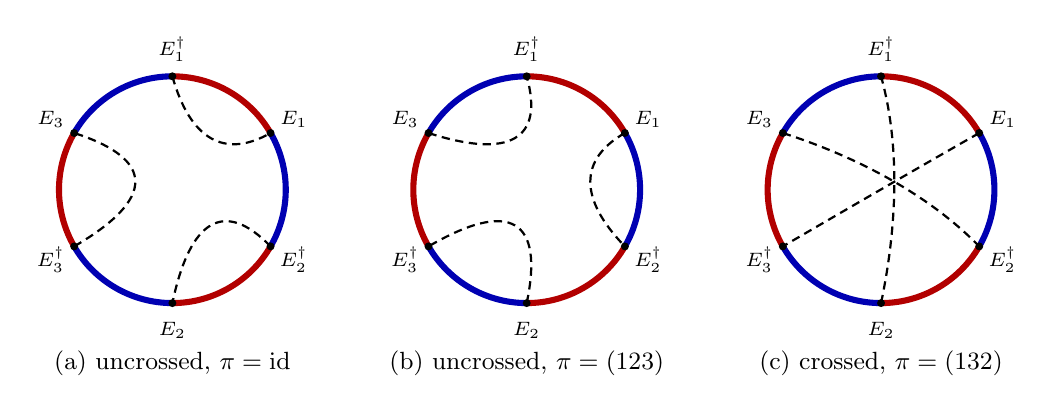
\begin{tikzpicture}[scale=0.9]
\foreach \X/\lab/\pairs in {0/{(a) uncrossed, $\pi=\mathrm{id}$}/{1/2,3/4,5/6},
                              5/{(b) uncrossed, $\pi=(123)$}/{2/3,4/5,6/1},
                              10/{(c) crossed, $\pi=(132)$}/{2/5,6/3,4/1}} {
  \begin{scope}[shift={(\X,0)}]
    % boundary: points k at angle 90-60(k-1)
    \foreach \k in {1,...,6} { \coordinate (p\k) at ({90-60*(\k-1)}:1.6); }
    % segments: G between (1,2),(3,4),(5,6); P between (2,3),(4,5),(6,1)
    \draw[line width=2.2pt,red!70!black] (90:1.6) arc (90:30:1.6);
    \draw[line width=2.2pt,red!70!black] (-30:1.6) arc (-30:-90:1.6);
    \draw[line width=2.2pt,red!70!black] (-150:1.6) arc (-150:-210:1.6);
    \draw[line width=2.2pt,blue!70!black] (30:1.6) arc (30:-30:1.6);
    \draw[line width=2.2pt,blue!70!black] (-90:1.6) arc (-90:-150:1.6);
    \draw[line width=2.2pt,blue!70!black] (150:1.6) arc (150:90:1.6);
    \foreach \a/\b in \pairs { \draw[thick,densely dashed] (p\a) .. controls ($0.35*(p\a)+(0.25,0.15)$) and ($0.35*(p\b)+(0.25,0.15)$) .. (p\b); }
    \foreach \k/\nm in {1/{E_1^\dagger},2/{E_1},3/{E_2^\dagger},4/{E_2},5/{E_3^\dagger},6/{E_3}} {
      \fill (p\k) circle (1.6pt); \node at ({90-60*(\k-1)}:1.98) {\scriptsize $\nm$}; }
    \node at (0,-2.45) {\small \lab};
  \end{scope}}
\end{tikzpicture}
\caption{Three of the six Wick contractions of $E_\eta\tr\Dc^3$, drawn as matter-chord diagrams (dashed). Blue
segments are zero-temperature (BPS) segments; red segments are the time-integrated propagation in the charged sector.
(a) Three $G$-faces of size 1 give $t_1^3$. (b) One $G$-face of size 3 gives $t_3$. (c) The single crossed
contraction.}
\label{fig:diagrams}
\end{figure}

\subsection{Uncrossed diagrams sum to a free compound Poisson law}

\begin{proposition}[Free compound Poisson]\label{prop:fcp}\COND\
Assume the chord rules for uncrossed matter correlators: each face of an uncrossed diagram carries a single energy, and
each matter chord between faces at energies $\phi,\phi'$ contributes the two-point kernel of \S\ref{sec:asc}
(BINT~\cite{BINT}; BLY~\cite[\S5]{BLY} for $\mathcal N=2$). Then the uncrossed part of $E_\eta\tr\Dc^m$ equals
$\sum_{\pi\in NC(m)}\prod_{G\text{-faces }F}t_{|F|}$, with
\begin{equation}\label{eq:tk}
t_k=\frac1b\Tr S^k,\qquad S=G^{1/2}\Vc G^{1/2}\ \text{diagonal in energy},\qquad
S(\phi)=g(\phi)=\frac{b\,c_0}{D_{\rm in}}\,\frac{A(\phi)}{\kappa\Lambda_{\sI}(\phi)} ,
\end{equation}
where $\Vc=E_\eta[E\,P\,E^\dagger]$ and $D_{\rm in}=\binom{N}{F+2}$. This is the moment--cumulant formula of free
probability with free cumulants $\kappa_k(\Dc)=t_k$. Without crossed diagrams, $\Dc$ is therefore distributed as a free
compound Poisson law: rate $r=e_{F+2}/b_F$, and jump distribution $g(\phi)$ with $\phi$ drawn from the normalized
density $\rho_B$. The same holds for the $g$ family.
\end{proposition}

\begin{proof}[Sketch]
\begin{itemize}\itemsep1pt
\item A $P$-face is a region in which every boundary segment is an infinitely long zero-temperature evolution at charge
  $\sout$. That projects the face's single energy onto the unique zero mode $\Psi_{\sout}$. The face is therefore rank
  one: it contributes the BPS density $b$ and no further dependence on the BPS state.
\item A $G$-face with $k$ integrated segments is bounded by $k$ matter chords, each joining it to a $P$-face. Each chord
  contributes $A(\phi)$ by Theorem~\ref{thm:asc}, and each segment contributes $\int d\tau\,e^{-\tau\kappa\Lambda}=1/(\kappa\Lambda)$.
\item Summing the face energy over the $\mathcal B$-family states, $D_{\rm in}\rho_B(\phi)d\phi$, gives
  $\Tr S^k$ with $S$ as in~\eqref{eq:tk}. The normalization uses $E_\eta\langle h|E^\dagger E|h\rangle=c_0$ and
  $\int f=1$.
\item Faces of an uncrossed diagram are $G$-faces for the cycles of $\pi$ and $P$-faces for the Kreweras complement.
  With the normalized trace this is the free moment--cumulant formula.
\end{itemize}
\end{proof}

The law in Proposition~\ref{prop:fcp} is also that of $Z^\dagger SZ$, where $Z$ is an $e\times b$ matrix of i.i.d.\
Gaussians with variance $1/b$. Its atoms, of mass $1-r$ when $r<1$, are the refined rank bound of~\cite[\S8]{prog1013}.
Two exact finite-$N$ identities hold without any chord input \DER:
\begin{equation}\label{eq:exactmoments}
E_\eta\tr\Dc=\tfrac1b\Tr S=\tr\Dbar,\qquad
E_\eta\tr\Dc^2=\tr\Dbar^2+\tfrac1b\Tr S^2,\qquad \Dbar\equiv E_\eta\Dc=2\textstyle\sum_IP\psi_IG\psi_I^\dagger P .
\end{equation}
Both are reproduced by the separable model $X=S^{1/2}ZC^{1/2}$ with $C=\Dbar/t_1$. The chord theory says $C=\one$
($P$-faces are rank one). It also says $S$ is diagonal in energy, since $G$-faces carry one energy. At finite $N$ the
second statement holds to $98.5$--$99.8\%$ of $\|S\|_F^2$ (Table~\ref{tab:t1}). The first fails: the eigenvalues of
$\Dbar$ spread by $12$--$42\%$ (\S\ref{sec:hetero}).

\subsection{Crossed diagrams}\label{sec:crossed}

A crossed diagram needs the matter--matter crossing (R-matrix) of the $\mathcal N=2$ chord theory. BINT~\cite{BINT}
constructed this for $\mathcal N=0$. BLY set up the $\mathcal N=2$ one-particle Hilbert space but did not evaluate a
crossed correlator. We therefore measure the crossed contribution directly \NUM. Take three independent Gaussian
coupling vectors $\alpha,\beta,\gamma$ and $X_v=G^{1/2}E_vV_b$. Then
\[
\tfrac1b\Tr\big[(X_\gamma^\dagger X_\alpha)(X_\beta^\dagger X_\gamma)(X_\alpha^\dagger X_\beta)\big]
\]
is an unbiased estimator of the crossed term of $E_\eta\tr\Dc^3$ alone, because each vector is contracted only with
itself. The same construction for the identity and full-cycle contractions reproduces their exact values $\tr\Dbar^3$
and $\frac1b\Tr S^3$, which validates the estimator. Table~\ref{tab:crossing} shows that the crossed term is between
$-0.5\%$ and $+0.2\%$ of the third moment and shrinks with $\Np$.

\begin{table}[ht]
\centering\small
\caption{The crossed matter-chord diagram as a fraction of $E_\eta\tr\Dc^3$ (two realizations per size; statistical
errors $\pm0.02\%$).}
\label{tab:crossing}
\setlength{\tabcolsep}{4pt}
\begin{tabular}{lccccc}\toprule
$\Np$ & 10 & 11 & 12 & 13 & 14\\\midrule
$h$ family & $-0.44\%$ & $+0.04\%,\,-0.02\%$ & $-0.14\%,\,-0.17\%$ & $+0.07\%,\,+0.04\%$ & $+0.12\%,\,+0.11\%$\\
$g$ family & $-0.43\%,\,-0.51\%$ & $-0.37\%,\,-0.39\%$ & $-0.15\%,\,-0.16\%$ & $-0.10\%,\,-0.08\%$ & $+0.09\%,\,+0.13\%$\\\bottomrule
\end{tabular}
\end{table}

%=====================================================================
\section{Gravity versus exact at \texorpdfstring{$\Np=10$--$16$}{N'=10-16}}\label{sec:tests}
%=====================================================================

\subsection{An error budget}

For each realization we compute five versions of the first-order spectrum. Each step changes one ingredient.
\begin{itemize}\itemsep1pt
\item \emph{exact}: the spectrum of $\Dc$ for the realization's own $\eta$ (identical to the first-order data
  of~\cite{prog1013}), and its average over $24$ further independent draws of $\eta$;
\item \emph{planar, exact inputs}: the separable model with the exact $S$ and $C=\Dbar/t_1$. This keeps the exact
  first two moments and drops everything else;
\item \emph{factorized}: the same with $C=\one$ (rank-one $P$-faces);
\item \emph{chord}: the population of $S$ from~\eqref{eq:tk}, with $C=\one$;
\item \emph{chord, rescaled}: the chord population rescaled to the exact $t_1$.
\end{itemize}
Table~\ref{tab:budget} and Figure~\ref{fig:W1} give the result, with the decoder's $W$ for reference.

\begin{table}[ht]
\centering\small
\caption{First-order heterogeneity $\Wone$ ($b$-weighted over both families) and $T_2^{(1)}$. ``Exact'' is the mean over
the 13 realizations of~\cite{prog1013} (6 at $\Np=15$, 2 at $\Np=16$). The models use 4, 4, 4, 4, 4, 3 and 1
realizations respectively. Every model column is a mean over realizations with standard error $\le0.0005$. The last
column is the decoder's $W$~\cite[Tables 5--6]{prog1013}; $^\ast$exact decoder on the two pre-registered $\Np=16$
realizations, $\Wone$ plus the measured residual.}
\label{tab:budget}
\setlength{\tabcolsep}{4.5pt}
\begin{tabular}{lccccccc}\toprule
$\Np$ & $\Wone$ exact & planar, exact inputs & factorized & chord & chord/exact & $T_2^{(1)}$ exact / chord & $W^\dec$\\\midrule
10 & 0.0587 & 0.0628 & 0.0623 & 0.0612 & 1.043 & 0.702 / 0.691 & 0.0666\\
11 & 0.0897 & 0.0947 & 0.0947 & 0.0967 & 1.078 & 0.625 / 0.608 & 0.0891\\
12 & 0.0838 & 0.0890 & 0.0893 & 0.0901 & 1.075 & 0.637 / 0.615 & 0.0897\\
13 & 0.1107 & 0.1161 & 0.1170 & 0.1202 & 1.086 & 0.565 / 0.545 & 0.1083\\
14 & 0.1045 & 0.1098 & 0.1105 & 0.1123 & 1.075 & 0.568 / 0.552 & 0.1085\\
15 & 0.1264 & 0.1314 & 0.1325 & 0.1365 & 1.080 & 0.525 / 0.494 & 0.123\\
16 & 0.1203 & 0.1242 & 0.1251 & 0.1281 & 1.065 & 0.535 / 0.502 & 0.124$^\ast$\\
\bottomrule\end{tabular}
\end{table}

\begin{figure}[t]
\centering
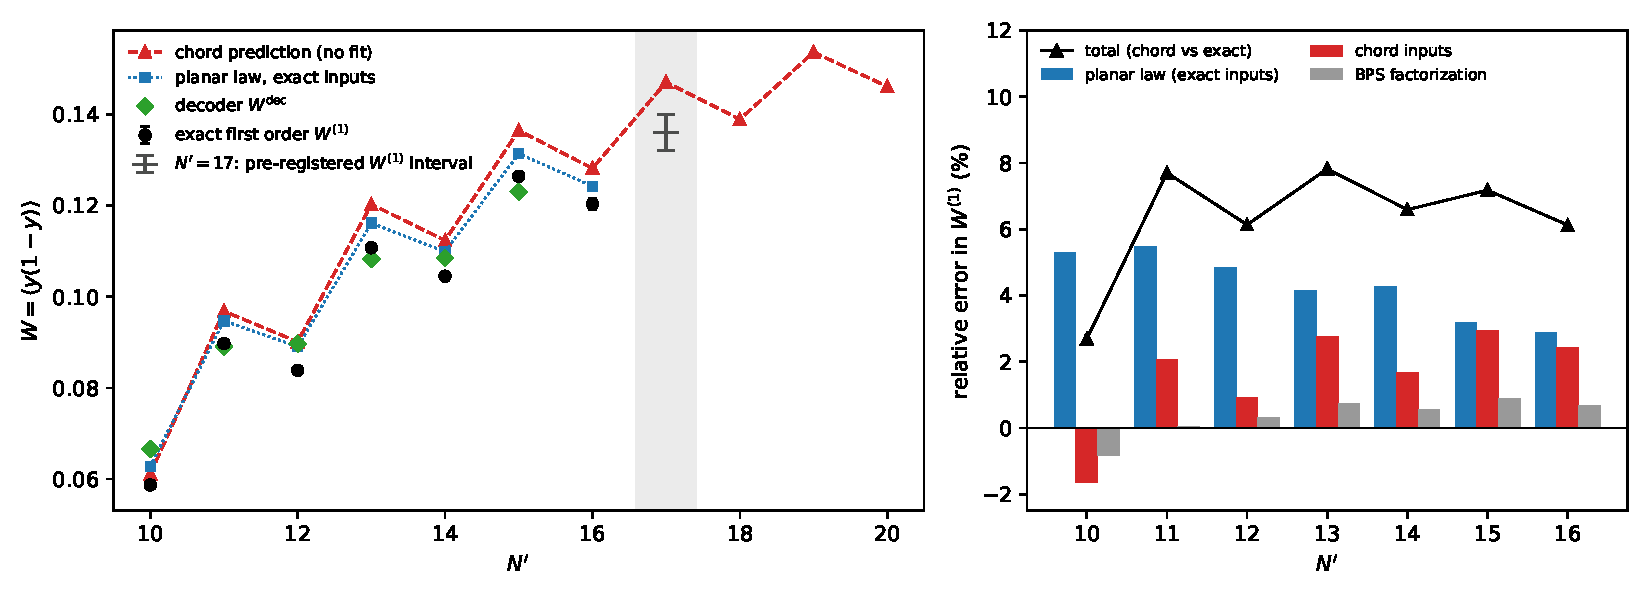
\includegraphics[width=\textwidth]{progress_2026-10-14_figs/fig_W1.pdf}
\caption{(a) First-order heterogeneity: exact (black), chord prediction with no fit (red), planar law with exact inputs
(blue), and the decoder's $W$ (green). The shaded band is the pre-registered $\Np=17$ test (\S\ref{sec:N17}).
(b) Error budget of the chord prediction relative to the exact first order: planar law, chord inputs and BPS
factorization, with their total.}
\label{fig:W1}
\end{figure}

The budget breaks down as follows \NUM.
\begin{enumerate}\itemsep2pt
\item \textbf{The planar law with exact inputs is $3$--$5\%$ high in $W$}: $+5.4\%$ at $\Np=10$, falling to $+3.2\%$
  at $15$ and $+2.9\%$ (one realization) at $16$. It is accurate for $T_2$. The difference sits at small $\sigma^2$, which $W$ weights
  heavily ($w(s)$ peaks at $s=0.17$; Figure~\ref{fig:sigma2}). The exact spectrum has a softer lower edge: more weight
  at $\sigma^2\lesssim0.03$, and at $\Np=13$--$14$ also the deterministic atom excess of~\cite[\S8]{prog1013}. This is
  not a crossed-diagram effect (Table~\ref{tab:crossing}). Nor is it the inner-level structure: at $\Np=10$, giving every
  inner energy eigenstate its own independent couplings (keeping each row's covariance exactly) restores the planar
  edge (1\% quantile $0.025$--$0.037$ against $0.015$--$0.027$ exact). The softness comes from the fact that all matrix
  elements share the same $\binom N2$ couplings. Its decrease with $\Np$ is consistent with that.
\item \textbf{The chord inputs add $1$--$3\%$ to $W$} and lower $T_2^{(1)}$ by $2$--$6\%$. This is the finite-$p$
  spectrum of \S\ref{sec:time}. Rescaling the chord population to the exact $t_1$ changes $W$ by at most $1\%$ (for example
  $0.1376$ instead of $0.1365$ at $\Np=15$). $W$ is insensitive to the overall scale and sensitive to the shape.
\item \textbf{BPS factorization costs less than $1\%$ in $W$}, although $\Dbar$ is far from $\propto\one$. At these sizes
  $r=e/b\simeq0.4$--$1.3$, so the intrinsic spread of the free law dominates.
\end{enumerate}
At $\Np=10$ the first two errors partly cancel. Elsewhere they add, to $+7$--$9\%$.

\begin{figure}[t]
\centering
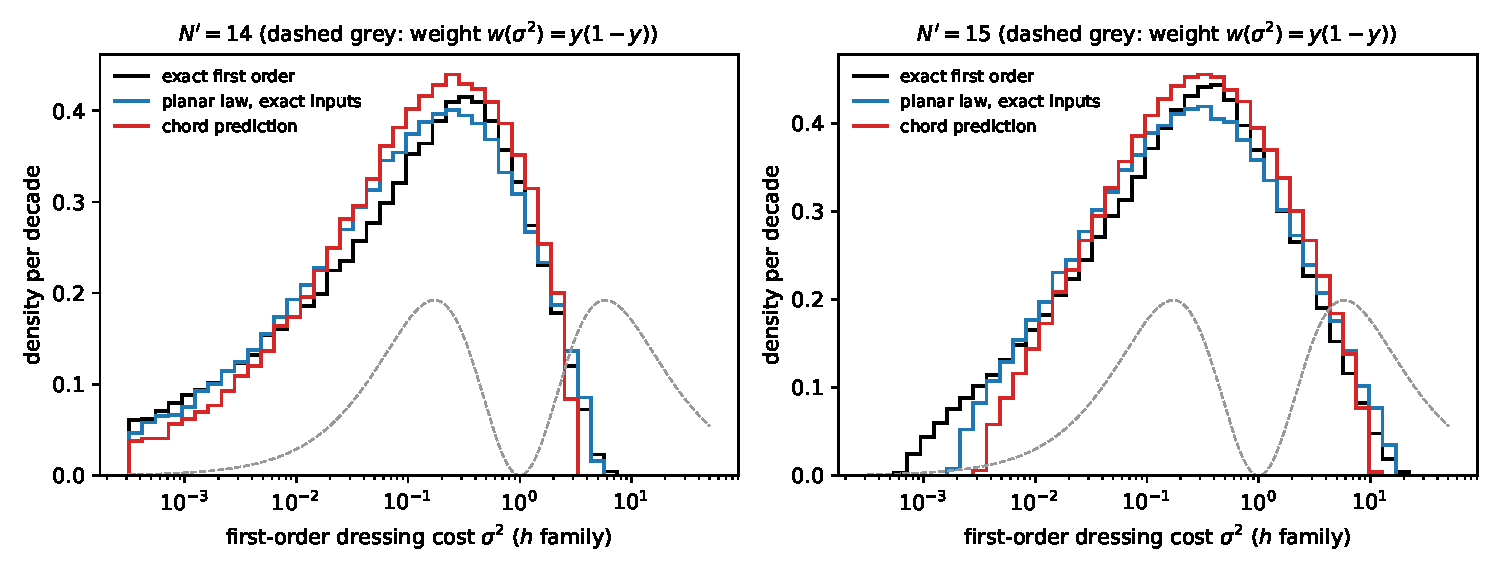
\includegraphics[width=\textwidth]{progress_2026-10-14_figs/fig_sigma2.pdf}
\caption{Distribution of first-order dressing costs ($h$ family, one realization, several $\eta$ draws). The exact
spectrum (black) has more weight at the smallest $\sigma^2$ than the planar law with exact inputs (blue) and the chord
prediction (red). The dashed grey curve is the weight $w(\sigma^2)=y(1-y)$ that enters $W$.}
\label{fig:sigma2}
\end{figure}

\subsection{Consequences for the decoder}

Replace $\Wone$ by its chord value in the prediction $T_4^\dec\approx T_2^\dec-\Wone$ of~\cite{prog1013}. The errors in
$T_4$ become $+0.005$, $-0.008$, $-0.000$, $-0.012$, $-0.004$, $-0.014$ for $\Np=10$--$15$. With BLY's chord $T_2$ as
well~\cite[\S9.3]{prog1013}, the prediction contains no input from the $\Np$-mode model and no fit. Its errors are
$+0.016$, $-0.004$, $+0.004$, $-0.015$, $-0.006$, $-0.022$, at most $4\%$ of $T_4$. The localization predicted from the
chord $W$ is $0.038$, $0.030$, $0.041$, $0.031$, $0.043$, $0.032$, against the measured $0.032$, $0.038$, $0.042$,
$0.043$, $0.047$, $0.045$. That is within $1$--$8\%$ at $\Np=12$ and $14$, and $20$--$30\%$ low at odd $\Np$. At odd
$\Np$ the chord excess in $\Wone$ adds to the negative first-order residual $W^\dec-\Wone$ of~\cite{prog1013}.

%=====================================================================
\section{A pre-registered test at \texorpdfstring{$\Np=17$}{N'=17}}\label{sec:N17}
%=====================================================================

\PRE\ The next size is $\Np=17$: an old model with $N=16$ modes, $F=8$, $b_8=4374$, $b_7=2187$ and $e_{10}=7449$ inner
exact forms. Before computing anything at this size, we wrote down predictions in
\path{results/data/chord_dressing_2026-10-14/prereg_N17.json} and committed them (commit \texttt{097cd6e}). They use
only the chord theory and the calibration at odd $\Np=11$, $13$, $15$. The parameter-free chord values are
$\Wone=0.1470$, $T_2^{(1)}=0.4520$, and $t_1=0.945$ ($h$) and $0.246$ ($g$). At odd $\Np$ the ratio exact/chord of
$\Wone$ has been $0.927$, $0.921$, $0.926$. It is stable because two errors move in opposite directions: the planar
error decreases ($+5.5$, $+4.1$, $+3.2\%$) while the chord-input error increases ($+2.1$, $+2.8$, $+3.0\%$).
Table~\ref{tab:prereg} lists the predictions. The protocol fixes the realizations (seeds 9000 and 9001, couplings as
in~\cite{prog1013}), the command, and the summary statistic: the mean over the two realizations of the first-order
spectra for the realizations' own couplings.

\begin{table}[ht]
\centering\small
\caption{Pre-registered predictions for $\Np=17$ (\texttt{prereg\_N17.json}). ``Chord'' is the parameter-free value; the
intervals combine it with the odd-$\Np$ calibration, the realization-to-realization scatter and the observed trends.}
\label{tab:prereg}
\begin{tabular}{@{}l>{\raggedright\arraybackslash}p{0.43\textwidth}cc@{}}\toprule
& Quantity & Chord & Pass interval\\\midrule
P1 & $\Wone$, exact first order & $0.1470$ & $[0.132,\,0.140]$\\
P2 & $\Wone_{\rm chord}/\Wone_{\rm exact}$ & -- & $[1.03,\,1.12]$\\
P3 & $T_2^{(1)}$, exact first order & $0.4520$ & $[0.463,\,0.513]$\\
P4 & $t_1$, $h$ family & $0.945$ & $[0.90,\,1.31]$\\
P5 & $t_1$, $g$ family & $0.246$ & $[0.230,\,0.290]$\\
P6 & exact first-order atoms & 0 & $0$\\
P7 & planar-law error in $W$ & -- & $[1.0,\,4.5]\%$\\
P8 & chord-input error in $W$ & -- & $[1.5,\,4.5]\%$\\
P9 & diagonal fraction of $S$ & $1$ & $\ge0.990$ ($h$), $\ge0.980$ ($g$)\\
P10 & spread of $\operatorname{spec}\Dbar$ (\S\ref{sec:hetero}) & $0$ & $[0.33,\,0.50]$ ($h$), $[0.12,\,0.20]$ ($g$)\\\bottomrule
\end{tabular}
\end{table}

\paragraph{Status.} The test has not been run at the time of writing. It is the first computation to do next. The
memory-lean code peaked at about $2$\,GB at $\Np=16$. The dominant arrays grow by factors of $4$--$7$ from $\Np=16$ to
$17$, so we expect about $10$\,GB, to be measured under the watchdog.

%=====================================================================
\section{BPS heterogeneity of the dressing cost}\label{sec:hetero}
%=====================================================================

\subsection{What the chord theory misses}

In the chord theory every $P$-face is rank one. The averaged dressing operator $\Dbar=E_\eta\Dc$ is therefore
proportional to the identity: every BPS state has the same mean dressing cost. At finite $N$ this fails
(Table~\ref{tab:hetero}, Figure~\ref{fig:hetero}a). The eigenvalues of $\Dbar$ spread by $22$--$42\%$ in the $h$ family
and $12$--$16\%$ in the $g$ family, with no decrease from $\Np=10$ to $16$. At these sizes the spread costs less than
$1\%$ in $\Wone$ (\S\ref{sec:tests}), because the intrinsic spread of the free law dominates. That intrinsic spread
shrinks once $r=e/b\gg1$, however, and the BPS heterogeneity would then control $W$. Its fate decides whether the chord
description survives at large $N$.

The heterogeneity is a late-time effect. By~\eqref{eq:c0}, $K(\tau)=P\,E_\eta[E^\dagger e^{-\tau H_0}E]\,P$ is exactly
proportional to $P$ at $\tau=0$. Its relative spread grows from about $1.5\%$ at $\tau E_{\rm med}=0.1$ to $12\%$ at $1$
and $50$--$75\%$ at $10$ (Figure~\ref{fig:hetero}b). Correspondingly, the lowest $5\%$ of the inner levels carry
$31$--$89\%$ of the variance of $\Dbar$.

It is not a pair-dependent energy cost. If creating the pair $(ij)$ simply cost a pair-dependent energy, $\Dbar$ would
be a weighted sum of hole-pair projectors, $\sum_{i<j}g_{ij}\,P(1-n_i)(1-n_j)P$. A least-squares fit of this form
explains only $4$--$18\%$ of the variance.

\subsection{A sum rule}

\begin{proposition}[Single-fermion sum rule]\label{prop:sumrule}\VER\
Let $c_i=\iota_i$ annihilate mode $i$, and let $E_i=\{Q_0,c_i\}=(\iota_i\omega_0)\wedge$ be the pair-creation
operator built from the old couplings $C_{i\cdot\cdot}$. On the BPS space of degree $F$,
\begin{equation}\label{eq:sumrule}
B_c+\sum_iP\,E_i^\dagger G\,E_i\,P=F\,P,\qquad B_c\equiv\sum_iP\,c_i^\dagger P_{F-1}c_i\,P .
\end{equation}
\end{proposition}

\begin{proof}
Because $\omega_0$ has odd degree, $\iota_i(\omega_0\wedge\beta)=(\iota_i\omega_0)\wedge\beta-\omega_0\wedge\iota_i\beta$,
so $\{c_i,Q_0\}=E_i$. Also $\{c_i,Q_0^\dagger\}=0$, since $Q_0^\dagger$ is a product of three annihilators. Take a
harmonic $\alpha$, so $Q_0\alpha=Q_0^\dagger\alpha=0$.
\begin{itemize}\itemsep1pt
\item $Q_0^\dagger c_i\alpha=-c_iQ_0^\dagger\alpha=0$, so $c_i\alpha$ is harmonic plus coexact:
  $c_i\alpha=P_{F-1}c_i\alpha+Q_0^\dagger\beta_i$.
\item $Q_0c_i\alpha=E_i\alpha$, so $Q_0Q_0^\dagger\beta_i=E_i\alpha$. Since $E_i\alpha$ is exact,
  $\|Q_0^\dagger\beta_i\|^2=\langle\alpha|E_i^\dagger GE_i|\alpha\rangle$.
\item By Pythagoras, $\|c_i\alpha\|^2=\|P_{F-1}c_i\alpha\|^2+\langle\alpha|E_i^\dagger GE_i|\alpha\rangle$.
\end{itemize}
Summing over $i$ with $\sum_ic_i^\dagger c_i=F$ on $\Lambda^F$ gives $\langle\alpha|(\text{LHS}-F)|\alpha\rangle=0$
for every BPS $\alpha$. The operator identity follows by polarization.
\end{proof}

For each old site, the dressing cost of that site's own pair operator and the BPS weight of its single-fermion
descendant add up to one. The added mode's $E$ is an operator of the same kind, with independent couplings. Numerically
the identity holds to $2.5\times10^{-14}$. The $\eta$-averaged $\Dbar$ correlates with the old-site version
$\sum_iPE_i^\dagger GE_iP$. Its traceless correlation with $B_c$ is therefore $-0.73$ to $-0.93$
(Table~\ref{tab:hetero}). The heterogeneity that the chord theory misses is thus the microstate dependence of
BPS-projected single-fermion two-point functions. Microstates whose single-fermion descendants stay BPS (large $B_c$)
are cheap to dress, and microstates whose descendants leave the BPS sector are expensive. This is the same kind of
quantity as the decoder's own heterogeneity.

\subsection{Incoherent and coherent parts}

Write $\Dbar=\sum_nM_n/E_n$, where $M_n=2\sum_IP\psi_I|n\rangle\langle n|\psi_I^\dagger P$ is the contribution of
inner level $n$. Each $M_n$ has rank at most $\binom N2$. If the $M_n$ were oriented at random (Haar) relative to each
other, free probability would give the eigenvalue variance $\sum_n[\tr M_n^2-(\tr M_n)^2]/E_n^2$. We call this the
\emph{incoherent} estimate; it is computed exactly from the Gram matrices of the vectors $P\psi_I|n\rangle$.

Table~\ref{tab:hetero} compares it with the observed spread. We look at the lowest $5\%$ of levels, where the variance
lives.
\begin{itemize}\itemsep1pt
\item The incoherent estimate is exact at $\Np=10$ and falls increasingly short: observed/incoherent $=1.00$, $1.09$,
  $1.15$, $1.37$, $1.41$, $1.72$ for $\Np=10$--$15$ ($h$).
\item The coherent share $1-(\text{incoherent}/\text{observed})^2$ grows from $0$ to $0.66$ ($h$) and to $0.54$ ($g$)
  (Figure~\ref{fig:hetero}c).
\item The effective number of contributing levels grows from $21$ to $365$, and the incoherent part shrinks as it
  should. The total stays flat because the coherent part takes over.
\end{itemize}
For the whole operator the comparison is complicated by the exact sum rule $\sum_nM_n=c_0P$, which makes the energy bins
anti-correlated.

\INTERP\ Two mechanisms are at work.
\begin{itemize}\itemsep1pt
\item An \emph{incoherent} one: a finite number of low-lying levels, each coupled through a low-rank channel. It decays
  like $1/N_{\rm eff}$ and is harmless for the chord theory at large $N$.
\item A \emph{coherent} one: the same BPS microstates are IR-heavy across many low-lying levels, and they are the ones
  with small single-fermion BPS weight. It does not decay in our window.
\end{itemize}
Its large-$N$ fate at fixed $p$ is the same open question as that of localization itself.

\begin{table}[ht]
\centering\small
\caption{BPS heterogeneity of $\Dbar$ (two realizations per size; at even $\Np$ the $g$ family equals the $h$ family by
Hodge duality). Columns: relative spread of $\operatorname{spec}\Dbar$, observed and incoherent estimate; the same for
the lowest $5\%$ of levels; coherent share of that variance; variance share of the lowest $5\%$ of levels; effective
number of contributing levels; traceless correlation of $\Dbar$ with the single-fermion BPS weight $B_c$; spread of
$\operatorname{spec}B_c$.}
\label{tab:hetero}
\setlength{\tabcolsep}{3.5pt}
\begin{tabular}{lcccccccc}\toprule
$\Np$, fam. & spread & incoh. & low 5\%: obs / incoh. & coh.\ share & var.\ share & $N_{\rm eff}$ & corr$(\Dbar,B_c)$ & spread $B_c$\\\midrule
10, $h$ & 0.216 & 0.356 & 1.75 / 1.75 & 0.00 & 0.31 & 21 & $-0.84$ & 0.146\\
11, $h$ & 0.396 & 0.389 & 1.27 / 1.16 & 0.17 & 0.71 & 37 & $-0.73$ & 0.336\\
11, $g$ & 0.120 & 0.271 & 1.04 / 1.02 & 0.04 & 0.37 & 28 & $-0.90$ & 0.068\\
12, $h$ & 0.253 & 0.283 & 1.05 / 0.91 & 0.25 & 0.63 & 72 & $-0.86$ & 0.164\\
13, $h$ & 0.411 & 0.306 & 1.00 / 0.73 & 0.48 & 0.83 & 116 & $-0.77$ & 0.345\\
13, $g$ & 0.142 & 0.206 & 0.83 / 0.71 & 0.27 & 0.57 & 106 & $-0.91$ & 0.077\\
14, $h$ & 0.246 & 0.218 & 0.89 / 0.63 & 0.50 & 0.74 & 252 & $-0.87$ & 0.161\\
15, $h$ & 0.417 & 0.248 & 0.91 / 0.53 & 0.66 & 0.89 & 365 & $-0.79$ & 0.339\\
15, $g$ & 0.156 & 0.162 & 0.71 / 0.48 & 0.54 & 0.76 & 373 & $-0.93$ & 0.082\\
\bottomrule\end{tabular}
\end{table}

\begin{figure}[t]
\centering
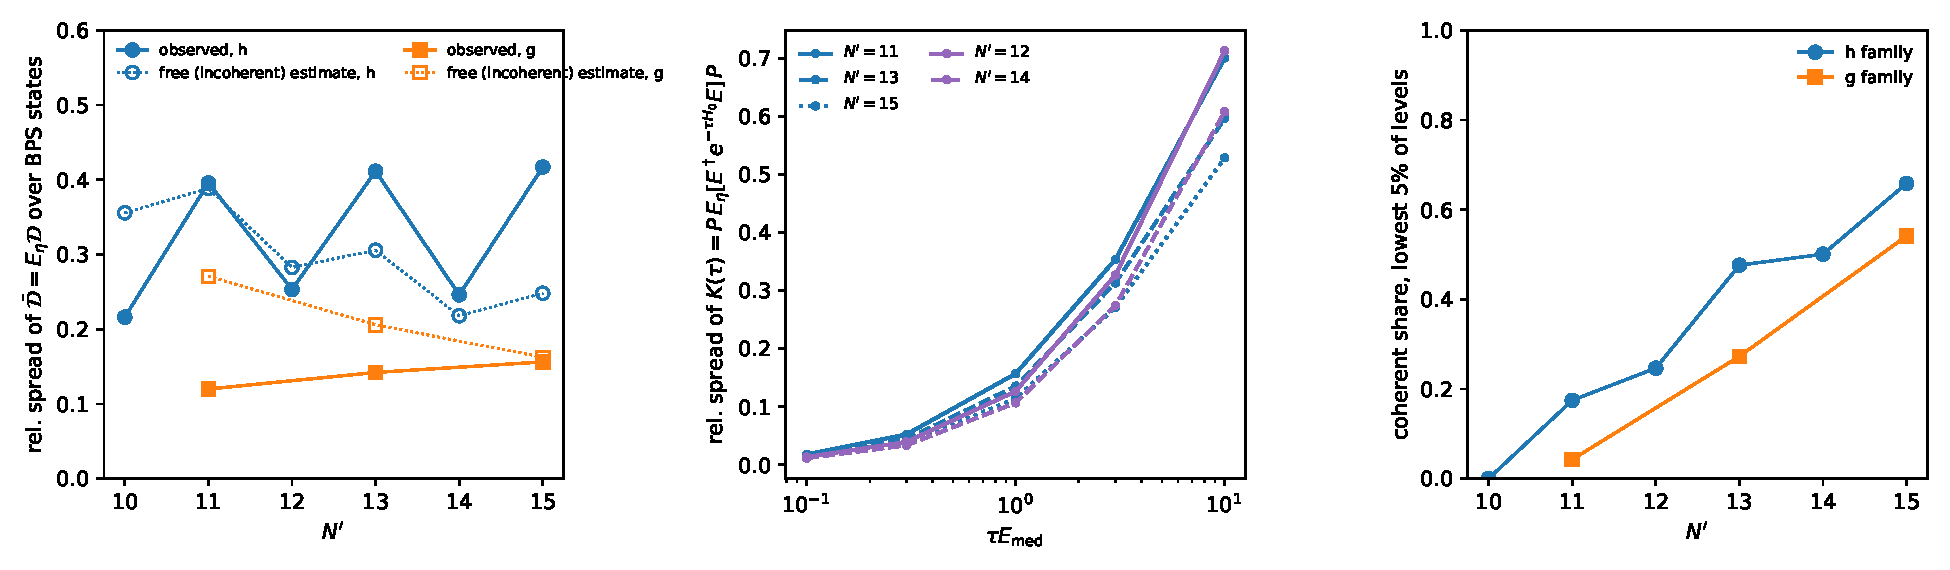
\includegraphics[width=\textwidth]{progress_2026-10-14_figs/fig_heterogeneity.pdf}
\caption{BPS heterogeneity of the averaged dressing cost. (a) Relative spread of the eigenvalues of $\Dbar$: observed
(filled) and incoherent (free-probability) estimate (open). (b) Spread of $K(\tau)$ against Euclidean time; it vanishes
at $\tau=0$. (c) Coherent share of the variance carried by the lowest $5\%$ of inner levels.}
\label{fig:hetero}
\end{figure}

%=====================================================================
\section{Discussion}\label{sec:discussion}
%=====================================================================

\subsection{What we have learned}

The dressing operator of the uplift problem is computable in the chord theory of $\mathcal N=2$ SYK, and three of its
ingredients are exact. Theorem~\ref{thm:asc} puts BLY's BPS-to-BPS and LMRS's BPS-to-continuum zero-temperature
two-point functions into a single Al-Salam--Chihara measure. The time integral is a ${}_2\phi_1$. The uncrossed
matter-chord diagrams sum to a free compound Poisson law.

At the sizes we can reach, the resulting gravitational prediction of the first-order heterogeneity is accurate to
$4$--$9\%$ with no fitted parameter, and the error budget accounts for the rest. Crossed diagrams are negligible. The
planar law has a slightly too hard lower edge, because all matrix elements share $\binom N2$ couplings. The finite-$p$
spectrum is broader than the double-scaled one.

The physics the chord theory misses at these sizes is BPS heterogeneity. An exact sum rule ties it to single-fermion
BPS-to-BPS weights. That is the localization question again, now in a different guise.

\subsection{Beyond accessible sizes}

Within the double-scaled model, the chord prediction extends to any size. With $r$ the inner-to-BPS dimension ratio,
the predictions are:
\begin{center}\small
\begin{tabular}{lccccccc}\toprule
$\Np$ & 17 & 18 & 19 & 20 & 24 & 30 & 40\\\midrule
$\Wone_{\rm chord}$ & 0.147 & 0.139 & 0.154 & 0.146 & 0.153 & 0.152 & 0.140\\
$r_h=e/b$ & 1.7 & 1.8 & 2.2 & 2.4 & 4.1 & 8.9 & 32\\
spread of the law, $\sqrt{t_2}/t_1$ ($h$) & 1.64 & 1.35 & 1.59 & 1.29 & 1.20 & 1.10 & 0.99\\\bottomrule
\end{tabular}
\end{center}
$\Wone_{\rm chord}$ peaks near $0.15$ at $\Np\approx24$--$30$ and then decreases slowly. Two effects compete: the free
law concentrates as $r$ grows exponentially, while $t_1$ grows like $N^{1/3}$. \INTERP\ These are predictions of the
double-scaled model, not of $p=3$ SYK, for three reasons.
\begin{itemize}\itemsep1pt
\item $\lambda\to0$ at fixed $p$ is the Schwarzian regime of DSSYK, whose coupling ($\alpha_S=1/8p^2$) differs from
  that of fixed-$p$ SYK (LMRS).
\item They are first order only.
\item They omit the coherent BPS heterogeneity of \S\ref{sec:hetero}, which would take over once $r\gg1$.
\end{itemize}

\subsection{Open problems and next steps}

\begin{enumerate}\itemsep2pt
\item \textbf{Run the pre-registered $\Np=17$ test} (\S\ref{sec:N17}), and complete the stopped $\Np=16$ runs
  (second realization of the decomposition; heterogeneity analysis).
\item \textbf{The coherent BPS heterogeneity.} Follow its share beyond $\Np=16$. Relate it directly to the decoder's
  localization: both $B_c$ and $Pn_eP$ are BPS-projected single-fermion quantities.
\item \textbf{The soft lower edge.} An operator-valued free-probability treatment, using the exact covariance of
  $X=\sum_I\eta_IG^{1/2}\psi_I^\dagger P$ with its few couplings, might capture it.
\item \textbf{The $\mathcal N=2$ matter--matter crossing.} It is needed for crossed diagrams here and for BLY's
  zero-temperature OTOC. Here it is not the bottleneck ($\le0.5\%$).
\item \textbf{Beyond first order.} Express the self-dressing and mixing steps of~\cite{prog1013} in chord language.
\end{enumerate}

\appendix

%=====================================================================
\section{Verification summary}\label{app:verify}
%=====================================================================

Every analytic statement was checked against an independent implementation, using the tests in
\path{tests/test_chord_dressing.py} (8 tests; the earlier test suites also pass).
\begin{itemize}\itemsep1pt
\item Ground-state amplitudes~\eqref{eq:gsrec}: equal to the $q$-Hermite closed form and to the zero mode of the
  transfer matrix, to $10^{-14}$.
\item The BBNR sign remark: direct action of $T$ on $\sum_n\alpha_n b_n$ (relative error $<10^{-9}$).
\item Theorem~\ref{thm:asc}: moments $\int f\Lambda^k$, $k=-2,\dots,3$, against the transfer matrix, to $10^{-15}$
  (test tolerance $10^{-8}$), at four parameter points; $f=\rho_BA$ and $\int f=1$.
\item Corollary~\ref{cor:bly}: point mass $=1-\int f=$ engine zero-mode weight $=$ BLY (4.14), to $10^{-12}$.
\item Proposition~\ref{prop:2phi1}: ${}_2\phi_1$ against quadrature, to $10^{-15}$.
\item Finite $N$:
  \begin{itemize}\itemsep0pt
  \item the lean code's first-order spectrum equals \texttt{OldModel}'s (\path{src/uplift.py}) to $10^{-9}$;
  \item $\Tr G\Vc=\Tr\Dbar$;
  \item the scatter construction of $\Vc$ equals the dense sum to $10^{-12}$;
  \item the second-moment identity~\eqref{eq:exactmoments} holds within sampling errors;
  \item the crossing estimator reproduces the exact identity and full-cycle terms.
  \end{itemize}
\item Proposition~\ref{prop:sumrule}: to $2.5\times10^{-14}$ at $\Np=10$--$13$.
\item The committed scripts reproduce the exploratory computations exactly (same seeds).
\end{itemize}

%=====================================================================
\section{Numerical methods and reproducibility}\label{app:repro}
%=====================================================================

\paragraph{Code.}
\begin{itemize}\itemsep1pt
\item \path{src/dssyk_n2.py}: closed forms (Theorem~\ref{thm:asc}, Corollary~\ref{cor:bly},
  Proposition~\ref{prop:2phi1}).
\item \path{src/chord_transfer.py}: transfer-matrix chord engine.
\item \path{src/chord_dressing.py}: chord predictions, finite-$N$ dressing machinery, crossing estimator, sum rule.
\end{itemize}

\paragraph{Scripts (with command-line parameters).}
\begin{itemize}\itemsep1pt
\item \path{scripts/run_chord_dressing.py} (\texttt{-{}-Np}, \texttt{-{}-seeds}, \texttt{-{}-neta}): error decomposition.
\item \path{scripts/run_chord_crossing.py}: crossed diagram.
\item \path{scripts/chord_dressing_predict.py}: chord predictions.
\item \path{scripts/analyze_bps_heterogeneity.py}: \S\ref{sec:hetero}.
\item \path{scripts/plot_chord_dressing.py}: figures and tables.
\end{itemize}

\paragraph{Data and parameters.} Everything is in \path{results/data/chord_dressing_2026-10-14/}, together with the
driver scripts \path{run_calibration.sh}, \path{run_crossing.sh} and \path{run_heterogeneity.sh}, logs and the
memory-watchdog log.
\begin{itemize}\itemsep1pt
\item Realizations: seeds $9000+k$, with couplings exactly as in~\cite{prog1013}. Seeds $9000$--$9003$ for
  $\Np=10$--$14$, $9000$--$9002$ at $15$, $9000$ at $16$.
\item $\eta$ draws: $24$ ($\Np\le14$), $12$ ($\Np=15$), $6$ ($\Np=16$).
\item Separable models: $3$ draws each.
\item Crossing estimator: $2000$, $1500$, $1000$, $600$, $300$ samples for $\Np=10$--$14$.
\item Chord predictions: $b_{\rm eff}=1500$, $3$ draws (finite-$b$ effects in $W$ below $10^{-4}$).
\end{itemize}

\paragraph{Memory.} All runs used the watchdog (\path{scripts/memwatch.py}). Peaks: about $2$\,GB for the calibration
(through $\Np=16$), $0.2$\,GB for the crossed diagrams, $0.8$\,GB for the predictions, and under $2$\,GB for the
heterogeneity analysis.

\paragraph{Not completed.} Two runs were stopped before finishing when this report was finalized: the second $\Np=16$
realization of the decomposition, and the $\Np=16$ heterogeneity analysis. The exploratory version of the first (seed 9001) gave
$\Wone=0.1190$ for its own couplings ($0.1182$ averaged over $6$ draws), $0.1240$ for the planar law with exact inputs
and $0.1281$ for the chord prediction, consistent with the realization shown.

\paragraph{Commits.} Code, data and pre-registration: \texttt{097cd6e}. This report: the following commit on branch
\texttt{t4-fourarc}.

\begin{thebibliography}{99}\small
\bibitem{CV} J.~Chryssanthacopoulos and D.~Vegh, \emph{Fortuity and fragility in supersymmetric SYK}, arXiv:2608.12160 (2026).
\bibitem{prog1013} \texttt{syk\_gravity} project, \emph{Progress report, 13 October 2026: the uplift map and the origin of localization}, \path{research/pdfs/progress_2026-10-13.pdf}.
\bibitem{BBNR} M.~Berkooz, N.~Brukner, V.~Narovlansky and A.~Raz, \emph{The double scaled limit of super-symmetric SYK models}, JHEP 12 (2020) 110, arXiv:2003.04405.
\bibitem{BLY} J.~Boruch, H.~W.~Lin and C.~Yan, \emph{Exploring supersymmetric wormholes in $\mathcal N=2$ SYK with chords}, JHEP 12 (2023) 151, arXiv:2308.16283.
\bibitem{LMRS} H.~W.~Lin, J.~Maldacena, L.~Rozenberg and J.~Shan, \emph{Looking at supersymmetric black holes for a very long time}, SciPost Phys.\ \textbf{14} (2023) 128, arXiv:2207.00408.
\bibitem{BINT} M.~Berkooz, M.~Isachenkov, V.~Narovlansky and G.~Torrents, \emph{Towards a full solution of the large $N$ double-scaled SYK model}, JHEP 03 (2019) 079, arXiv:1811.02584.
\bibitem{KLS} R.~Koekoek, P.~A.~Lesky and R.~F.~Swarttouw, \emph{Hypergeometric Orthogonal Polynomials and Their $q$-Analogues}, Springer (2010).
\bibitem{GR} G.~Gasper and M.~Rahman, \emph{Basic Hypergeometric Series}, 2nd ed., Cambridge University Press (2004).
\end{thebibliography}

\end{document}
